

\tikzset{every picture/.style={line width=0.75pt}} %set default line width to 0.75pt        

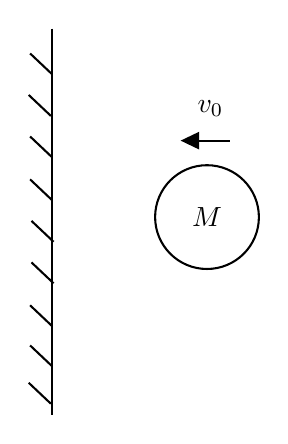
\begin{tikzpicture}[x=0.75pt,y=0.75pt,yscale=-1,xscale=1]
%uncomment if require: \path (0,244.3173065185547); %set diagram left start at 0, and has height of 244.3173065185547

%Straight Lines [id:da41391987557326315] 
\draw    (50.43,48.24) -- (50.43,234.24) ;


%Straight Lines [id:da8975629204988387] 
\draw    (50.43,70.24) -- (39.77,60.16) ;
\draw    (49.77,90.24) -- (39.1,80.16) ;
\draw    (50.43,110.24) -- (39.77,100.16) ;
\draw    (50.43,130.91) -- (39.77,120.83) ;


%Straight Lines [id:da3207421376516373] 
\draw    (51.1,150.91) -- (40.43,140.83) ;


%Straight Lines [id:da4433189705331644] 
\draw    (51.1,170.91) -- (40.43,160.83) ;


%Straight Lines [id:da1320019866862019] 
\draw    (50.43,191.58) -- (39.77,181.5) ;


%Straight Lines [id:da17396697635412584] 
\draw    (50.43,210.91) -- (39.77,200.83) ;


%Straight Lines [id:da7024410341299809] 
\draw    (49.77,228.91) -- (39.1,218.83) ;


%Shape: Circle [id:dp7508815890818632] 
\draw   (100,139) .. controls (100,125.19) and (111.19,114) .. (125,114) .. controls (138.81,114) and (150,125.19) .. (150,139) .. controls (150,152.81) and (138.81,164) .. (125,164) .. controls (111.19,164) and (100,152.81) .. (100,139) -- cycle ;
%Straight Lines [id:da41402643933373806] 
\draw    (114.31,102.16) -- (135.97,102.16) ;

\draw [shift={(112.31,102.16)}, rotate = 0] [fill={rgb, 255:red, 0; green, 0; blue, 0 }  ][line width=0.75]  [draw opacity=0] (8.93,-4.29) -- (0,0) -- (8.93,4.29) -- cycle    ;

% Text Node
\draw (126.67,86.67) node  [align=left] {$\displaystyle v_0$};
% Text Node
\draw (125,139) node  [align=left] {$\displaystyle M$};


\end{tikzpicture}